% % % % % % % % % % % % % % % % % % % % % % % % % % % % % % % % % % % % % % % %
% LaTeX4EI Template for Cheat Sheets                                Version 1.1
%
% Authors: Emanuel Regnath, Martin Zellner
% Contact: info@latex4ei.de
% Encode: UTF-8, tabwidth = 4, newline = LF
% % % % % % % % % % % % % % % % % % % % % % % % % % % % % % % % % % % % % % % %


% ======================================================================
% Document Settings
% ======================================================================

% possible options: color/nocolor, english/german, threecolumn
% defaults: color, english
\documentclass[english, threecolumn]{latex4ei/latex4ei_sheet}

% additional packages
\DeclareTextFontCommand{\emph}{\bfseries}
\usepackage{multirow} % for tables

% set document information
\title{How to Ace the Data Science Case Interview }
\author{LaTeX4EI}					% optional, delete if unchanged
\myemail{info@latex4ei.de}			% optional, delete if unchanged
\mywebsite{https://github.com/leoniewgnr/DataScienceCheatsheets}			% optional, delete if unchanged


% ======================================================================
% Begin
% ======================================================================
\begin{document}

\IfFileExists{git.id}{\input{git.id}}{}
\ifdefined\GitRevision\mydate{\GitNiceDate\ (git \GitRevision)}\fi

% Title
% ----------------------------------------------------------------------
\maketitle   % requires ./img/Logo.pdf


% Section
% ----------------------------------------------------------------------
\section{Understanding the Situation and Problem Statement}
\begin{sectionbox}
\begin{symbolbox}
Steps 1-4 are the steps to follow in a case interview. Step 5 gives more details on ML models.
\end{symbolbox}
    Define the business problem clearly: Take notes, repeat the problem and ask questions. 
\end{sectionbox}

\section{Data Collection and Preparation}
\begin{sectionbox}
    \subsection{Data Sources}
    \begin{itemize}
        \item Databases, APIs, files
        \item Social media networks
    \end{itemize}
    What data types are those?
    
    \subsection{Data Cleaning}
    \begin{itemize}
        \item Imputation or removal
        \item Z-score: How many standard deviations a specific value is from the mean $\rightarrow > 2$ ($< -2$)
        \item IQR: Difference between Q3 and Q1 (50\% of the data), upper limit: $Q3 + 1.5 \times IQR$
    \end{itemize}
    
    \subsection{Exploratory Data Analysis (EDA)}
    \begin{itemize}
        \item Visualization: Histograms, Scatterplots, correlation matrices
        \item Statistical analysis: Distribution, trends, relationships between variables
    \end{itemize}
    
    \subsection{Data Preparation}
    \begin{itemize}
        \item Min-Max or Z-standardization
        \item Relevant features
        \item Train, val, and test split
    \end{itemize}

    \subsection{What else to consider}
    \begin{itemize}
        \item Legal: GDPR, Anonymization
        \item Scalability: Fast datatypes (dask), PCA
    \end{itemize}
\end{sectionbox}


\section{Model Selection and Development}
\begin{sectionbox}
    
\subsection{Model Selection}
\textbf{Supervised Learning}: Algorithms that learn from labeled data (e.g., Regression, Classification).\\
\textbf{Unsupervised Learning}: Algorithms that learn from unlabeled data (e.g., Clustering, Dimensionality Reduction).\\
\textbf{Reinforcement Learning}: Algorithms that learn through reward and punishment.\\
\textbf{Bias-Variance Tradeoff}: Tradeoff between overfitting (high variance) and underfitting (high bias).\\
Bias: learn the wrong relationship\\
Variance: learns random relations that do not correlate with the data

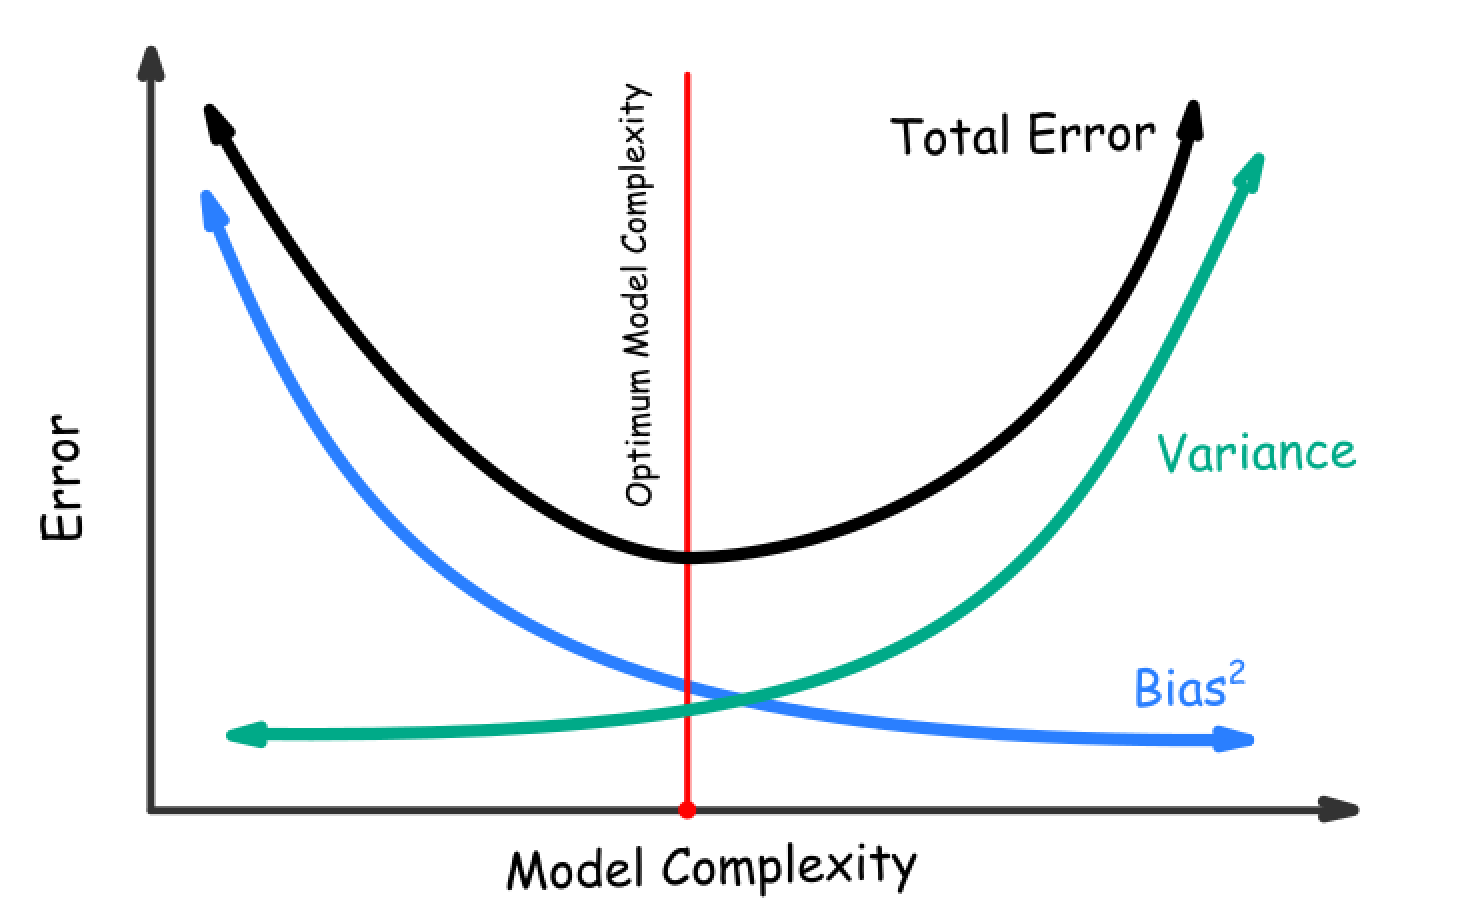
\includegraphics[width=0.45\textwidth]{img/biasvariance.png}
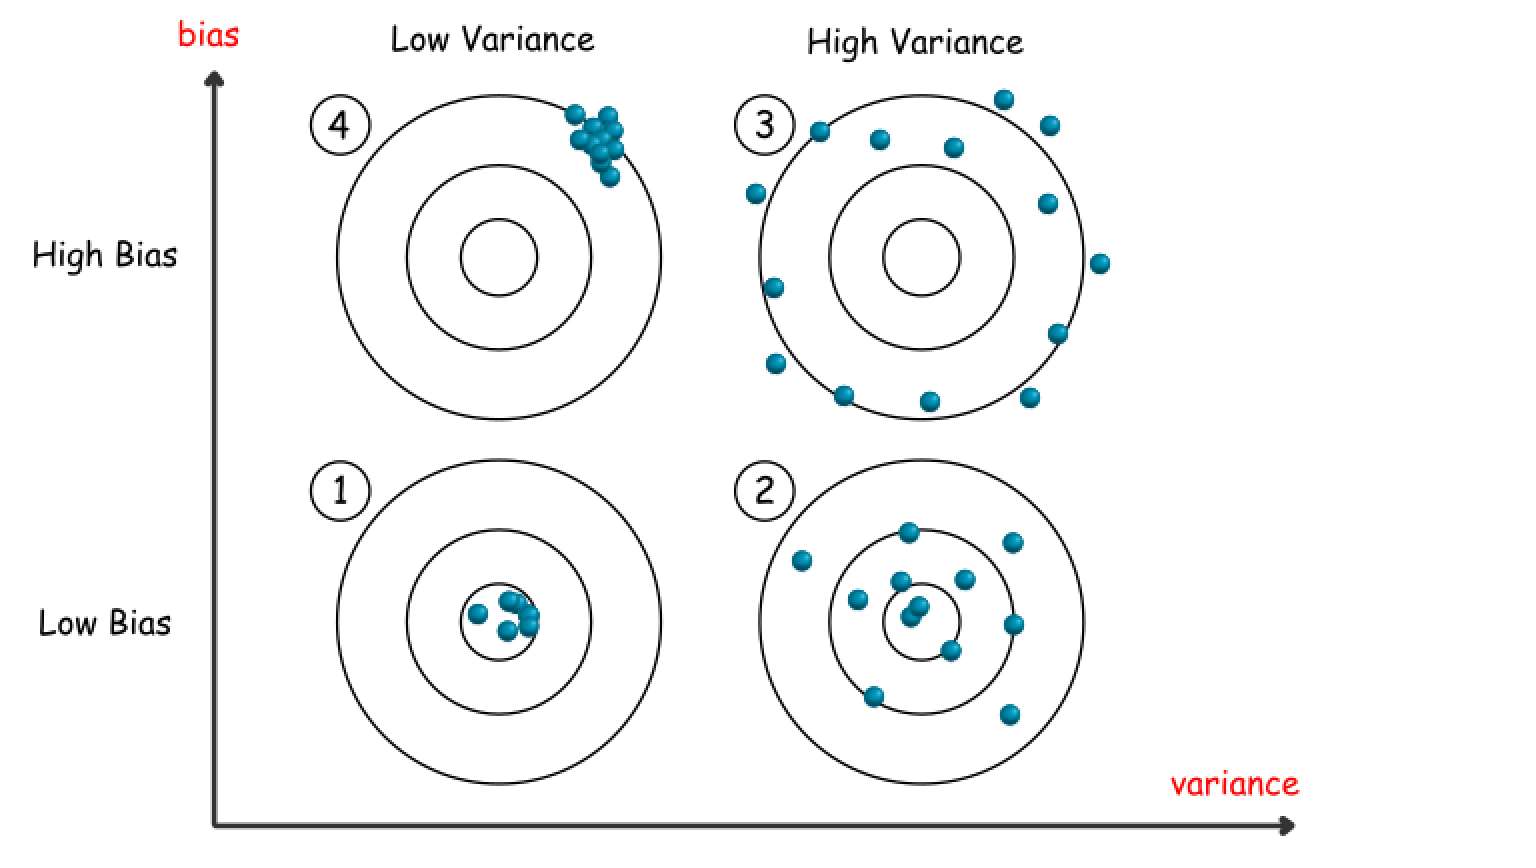
\includegraphics[width=0.45\textwidth]{img/biasmatrix.png}

\textbf{Cross-Validation:} Technique for avoiding overfitting by splitting the data into multiple folds.

\subsection{Model Development}
\textbf{Feature Engineering}: Selection and transf. of features to improve performance.\\
\textbf{Hyperparameter Tuning}: Optimization of parameters that are not learned from the data (e.g., Learning Rate).\\
\textbf{Ensemble Learning}: Combining multiple models to improve accuracy (e.g., Random Forest, Bagging, Boosting).\\
\textbf{Regularization}: Techniques to avoid overfitting (e.g., L1/L2 regularization).\\
\textbf{Loss Functions}: Functions to measure the error of a model (e.g., Mean Squared Error, Cross-Entropy).
\end{sectionbox}

\begin{sectionbox}
\subsection{Models}
\begin{tablebox}{>\raggedright p{0.1\linewidth} >\raggedright p{0.19\linewidth} p{0.19\linewidth} p{0.19\linewidth} p{0.19\linewidth}}
& \emph{Linear Regression} & \emph{Logistic Regression} & \emph{Decision Tree} & \emph{Random Forest} \\ \cmrule
Type & Supervised & Supervised & Supervised & Supervised \\
Target Variable & Continuous & Binary/Categorical & Both & Both \\
Expl. & Linear relationship between features and target. & Estimates probabilities for categorical target variable. & Splits data based on feature values. & Ensemble of decision trees for robustness. \\
Use Case & Price prediction, Trend analysis & Classification, Spam detection & Classification, Regression & Classification, Regression \\
Prereqs. & Linear relationship & Linear boundaries & None & None \\
Complex. & Low & Low & Medium & Medium \\
Params & Learning rate, Regularization & Learning rate, Regularization & Depth, Split criteria & Number of trees, Depth \\
Metric & RMSE, MAE & Accuracy, F1 & Accuracy, RMSE & Accuracy, RMSE \\
Interpret- ability & High & High & Medium & Medium \\
\end{tablebox}
\end{sectionbox}

\begin{sectionbox}
\begin{tablebox}{>\raggedright p{0.1\linewidth} >\raggedright p{0.19\linewidth} p{0.19\linewidth} p{0.19\linewidth} p{0.19\linewidth}}
& \emph{SVM} & \emph{K-NN} & \emph{K-Means} & \emph{Neural Networks} \\ \cmrule
Type & Supervised & Supervised & Unsupervised & Supervised \\
Target Variable & Binary/Categorical & Both & None & Both \\
Expl. & Finds the best separating line/plane between classes. & Classifies elements based on their neighbors. & Groups data into k similar clusters. & Simulates a neural network for complex patterns. \\
Use Case & Text classification, Face recognition & Recommendation systems, Classification & Customer segmentation, Anomaly detection & Image recognition, NLP \\
Prereqs. & Scaling, Labeling & Feature scaling & None & Large data set \\
Complex. & High & Low & Medium & High \\
Params & C, Kernel & Number of neighbors & Number of clusters & Learning rate, Neurons, Layers \\
Metric & Accuracy, F1 & Accuracy, RMSE & Silhouette Score, Inertia & Accuracy, F1 \\
Interpret- ability & Low & High & Medium & Low \\
\end{tablebox}
\end{sectionbox}

\begin{sectionbox}
\begin{tablebox}{>\raggedright p{0.1\linewidth} >\raggedright p{0.39\linewidth} p{0.39\linewidth}}
& \emph{Naive Bayes} & \emph{ARIMA} \\ \cmrule
Type & Supervised & Supervised \\
Target Variable & Categorical & Time series \\
Expl. & Uses Bayesian theory for classification. & Models time series through trend, seasonality, and noise. \\
Use Case & Text classification, Spam filter & Financial markets, Weather prediction \\
Prereqs. & Independent features & Stationarity \\
Complex. & Low & Medium \\
Params & Laplace smoothing & p, d, q parameters \\
Metric & Accuracy, F1 & RMSE, MAE \\
Interpret- ability & High & Medium \\
\end{tablebox}
\end{sectionbox}

\begin{sectionbox}
\subsection{Evaluation Metrics}
\subsubsection{Regression}
\textbf{Mean Squared Error (MSE)} $\frac{1}{n}\sum (y_i - \hat{y_i})^2$\\
\textbf{Sum of Squared Errors (SSE)} $\sum (y_i - \hat{y_i})$\\
\textbf{Total Sum of Squares (SST)} $\sum (y_i - \overline{y_i})$\\
\textbf{$R^2$ Score}: $1-\frac{SSE}{SST}$ ratio of explained variability in the data, not valid for nonlinear models, <0: worse than predicting just the mean \\

\subsubsection{Classification}
\textbf{Accuracy}: Ratio of correct predictions to the total number of predictions. BUT: problem with imbalanced classes $\rightarrow$ good for classification problems with balanced classes\\
\textbf{Precision}: $\frac{TP}{TP+FP}$ $\rightarrow$ideal if no FP (Spam detection: negative/no-spam mail is detected as positive/spam)\\
\textbf{Recall (TPR)}: $\frac{TP}{TP+FN}$ $\rightarrow$ ideal if no FN (Disease detection: positive/sick patient is detected as healthy/negative)\\
\textbf{F1-Score}: $2\frac{\text{precision} * \text{recall}}{\text{precision} + \text{recall}}$ $\rightarrow$ for imbalanced classes\\
\textbf{ROC-AUC}: Plot TPR vs FPR for different classification thresholds, aread under the curve = how likely the model differentiates positives vs negatives (1: perfect classification, 0.5: like random), not dependent on threshold, not always interpretable\\

\begin{tablebox}{lllll}
 &  & \multicolumn{2}{l}{\emph{Actual}} &  \\ \cline{3-4}
 &  & \multicolumn{1}{l|}{Positive} & Negative &  \\ \cline{3-4}
\multicolumn{1}{l|}{\multirow{2}{*}{\emph{Prediction}}} & \multicolumn{1}{l|}{Positive} & \multicolumn{1}{l|}{\begin{tabular}[c]{@{}l@{}}TP\\ Correct as positive\end{tabular}} & \begin{tabular}[c]{@{}l@{}}FP\\ Incorrect as positive\end{tabular} &  \\ \cline{2-4}
\multicolumn{1}{l|}{} & \multicolumn{1}{l|}{Negative} & \multicolumn{1}{l|}{\begin{tabular}[c]{@{}l@{}}FN\\ Incorrect as negative\end{tabular}} & \begin{tabular}[c]{@{}l@{}}TN\\ Correct as negative\end{tabular} & 
\end{tablebox}

\end{sectionbox}

\section{Implementation and Communication}
\begin{sectionbox}
\subsection{Implementation}
    \textbf{Version Control (e.g., Git)}: For collaborative work and tracking changes.\\
    \textbf{Continuous Integration / Continuous Deployment (CI/CD)}: Automatic testing and deployment of code.\\
    \textbf{Model Serving}: Hosting models for real-time access, e.g., via REST APIs.
    \item \textbf{Containerization (e.g., Docker)}: Packaging of software and dependencies for consistent execution.\\
    \textbf{Scaling}: Adjusting resources to load, e.g., through horizontal scaling.\\
    \textbf{Monitoring \& Logging}: Monitoring system performance and capturing important information.
        
\subsection{Communication}
    \textbf{Data Visualization}: Effective presentation of data using charts (e.g., Matplotlib, Seaborn).\\
    \textbf{Storytelling with Data}: Connecting analyses with a narrative structure to convey insights.\\
    \textbf{Interactive Dashboards (e.g., Tableau, Power BI, Dash)}: Creating interactive reports for end users.\\
    \textbf{Technical Documentation}: Clear and precise documentation of code, architecture, and decisions.\\
    \textbf{Non-Technical Communication}: Explaining technical concepts to a broader audience (e.g., stakeholders).\\
        \begin{itemize}
            \item ROI Analysis (Return on Investment): Evaluating how the results affect the business outcome.
            \item KPIs (Key Performance Indicators): Understanding and measuring the key metrics relevant to the business goal.
            \item Statistical Significance \& Confidence Intervals: Assessing the reliability of the results.
            \item Cost-Benefit Analysis: Weighing the implementation costs against expected benefits.
            \item Risk Assessment: Assessing potential risks or downsides of implementing the results.
            \item Scenario Analysis: Conducting "what-if" analyses to understand different business scenarios.
        \end{itemize}
    \textbf{Ethics and Compliance}: Understanding and adhering to legal and ethical guidelines (e.g., GDPR).
    
\subsection{Model Management}
    \subsubsection{Model Tracking (e.g., MLflow)} 
    Tracking experiments, models, and metrics.
    \subsubsection{A/B Testing}
    Comparing model versions to select the best.
    \paragraph{Procedure}
    \begin{enumerate}
        \item Randomly split the traffic (or data) into two groups: one served by model A and the other by model B.
        \item Measure the performance metric of interest (e.g., conversion rate, click-through rate, etc.) for both groups.
        \item Use statistical hypothesis testing to determine if the difference in performance is statistically significant.
    \end{enumerate}

\end{sectionbox}

\section{Machine Learning Models}
\begin{sectionbox}
\subsection{Linear Regression}
Most basic and widely used techniques in predictive modeling\\
linear relationship between the dependent variable and one or more independent continuous variables
\subsubsection{Assumptions}
\begin{itemize}
    \item Linear Relationship: Assumes that the relationship between the dependent and independent variables is linear.
    \item Independence: Observations are independent of each other.
    \item Homoscedasticity: Constant variance of errors.
    \item Normality: The errors follow a normal distribution.
\end{itemize}

\subsubsection{Equation}
\(y = \beta_0 + \beta_1 x_1 + \epsilon\), where \(y\) is the dependent variable, \(x_1\) is the independent variable, \(\beta_0\) is the y-intercept, \(\beta_1\) is the slope, and \(\epsilon\) is the error term.

\subsubsection{Training Parameters}
Learning Rate: For gradient descent optimization.\\
Regularization: To prevent overfitting.
\begin{itemize}
    \item Ridge Regularization (L2): $\|Y-X \beta\|^{2}+\lambda\|\beta\|^{2}$ $\rightarrow$ coefficients to almost zero (keeps all features), less computationally complex, better if predictors are highly correlated
    \item Lasso Regularization (L1): $\|Y-X \beta\|^{2}+\lambda\|\beta\|_{1}$ $\rightarrow$ some coefficients to zero (feature selection)
    \item Elastic net: combined
\end{itemize}

\subsubsection{Use-cases}
\begin{itemize}
    \item Price prediction
    \item Trend forecasting
    \item Risk assessment
\end{itemize}

\begin{tablebox}{p{0.4\textwidth} p{0.55\textwidth}}
\emph{Strengths} & \emph{Weaknesses} \\ \cmrule
Simple and interpretable &  Only captures linear relationships\\
Fast to model and predict & Sensitive to outliers\\
Works well on small datasets & Cannot handle multicollinearity (independent variables are highly correlated) well\\
\end{tablebox}

\subsubsection{Data Preprocessing}
\begin{itemize}
    \item Feature scaling: Often required.
    \item Missing values: Need to be handled.
    \item Categorical variables: One-Hot Encoding.
\end{itemize}

\subsubsection{Interpretability}
High; coefficients represent the change in the dependent variable for a one-unit change in an independent variable.

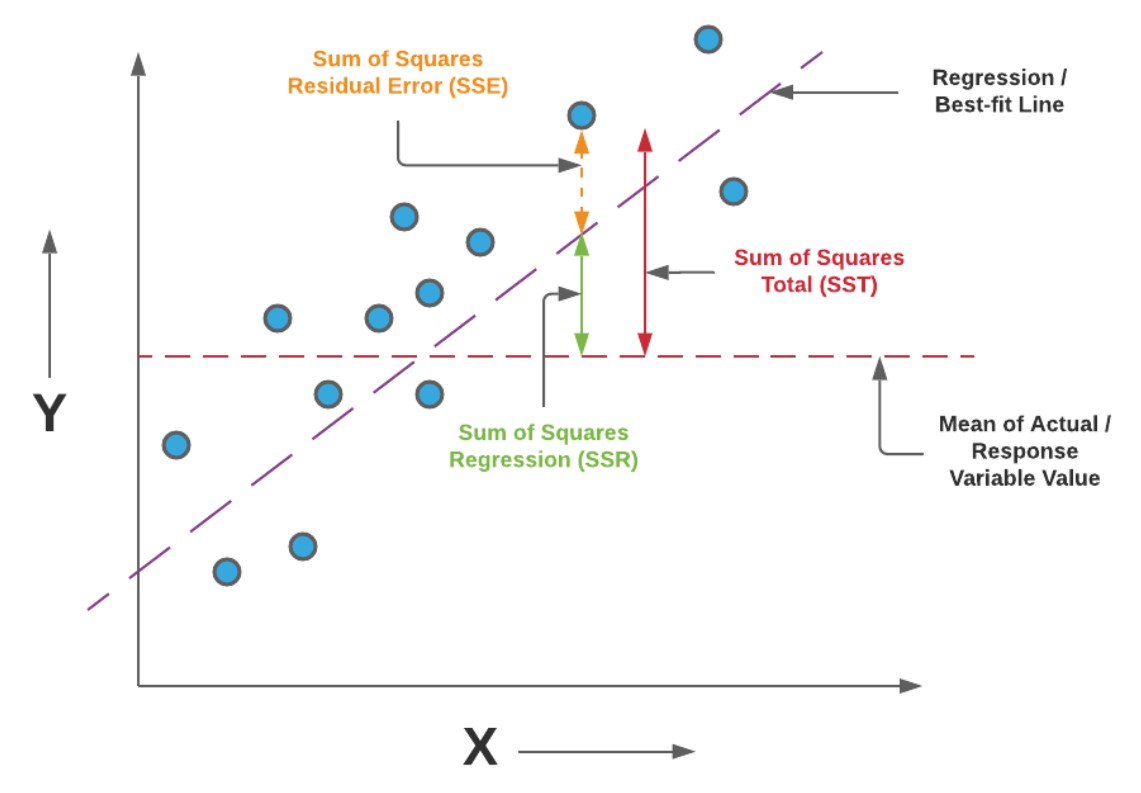
\includegraphics[width=0.6\linewidth]{img/linear-regression-f-statistics-definition.jpg}
\end{sectionbox}

\begin{sectionbox}
\subsection{Logistic Regression}
for classification problems, especially for binary outcomes\\
Transforms its output to lie in the range of 0 to 1 using the logistic function.

\subsubsection{Assumptions}
\begin{itemize}
    \item Linear Relationship: Assumes a linear relationship between the logit of the outcome and the predictor variables.
    \item Independence: Observations should be independent of each other.
    \item Large Sample Size: Needs a large sample size for maximum likelihood estimates to be truly asymptotic.
\end{itemize}

\subsubsection{Equation}
\( \ln\left(\frac{p}{1-p}\right) = \beta_0 + \beta_1 x_1 + \epsilon \), where \( p \) is the probability of the dependent event occurring, \( x_1 \) is the independent variable, \( \beta_0 \) is the intercept, \( \beta_1 \) is the slope, and \( \epsilon \) is the error term.

\subsubsection{Training Parameters}
\begin{itemize}
    \item Learning Rate: For optimization using methods like stochastic gradient descent.
    \item Regularization: To avoid overfitting, commonly used methods include L1 and L2 regularization.
\end{itemize}

\subsubsection{Use-cases}
\begin{itemize}
    \item Customer churn prediction
    \item Image classification
    \item Medical diagnosis
\end{itemize}

\begin{tablebox}{p{0.4\textwidth} p{0.55\textwidth}}
\emph{Strengths} & \emph{Weaknesses} \\ \cmrule
High interpretability & Not suitable for non-linear problems \\
Efficient to train & Sensitive to feature scale \\
Can provide calibrated probabilities & Prone to underfitting \\
\end{tablebox}

\subsubsection{Data Preprocessing}
\begin{itemize}
    \item Feature Scaling: Required for regularization and gradient descent.
    \item Missing Values: Must be addressed.
    \item Categorical Variables: Label encoding or one-hot encoding often used.
\end{itemize}

\subsubsection{Interpretability}
Coefficients signify the odds ratio for the given predictor variable. A coefficient greater than 1 represents increased odds of the outcome, while a coefficient less than 1 represents decreased odds.

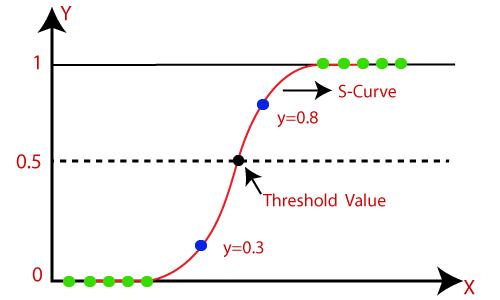
\includegraphics[width=0.5\linewidth]{img/logistic-regression-in-machine-learning.png}
\end{sectionbox}

\begin{sectionbox}
    \subsection{Decision Tree}
For both classification and regression tasks. \\
Decision trees work by splitting the dataset into subsets based on the most significant attributes, making decisions at every level.

\subsubsection{Assumptions}
\begin{itemize}
    \item None: One of the few algorithms that does not assume any underlying data distribution.
\end{itemize}

\subsubsection{Equation}
No single equation represents a decision tree. They are built using algorithms like ID3, C4.5, or CART, which use measures like Information Gain, Gain Ratio, or Gini Index to decide splits.

\subsubsection{Training Parameters}
\begin{itemize}
    \item Max Depth: Maximum depth of tree.
    \item Min Samples Split: Minimum number of samples required to split an internal node.
    \item Min Samples Leaf: Minimum number of samples required to be at a leaf node.
    \item Criterion: Metric used for splitting (Gini, Entropy)
    \begin{itemize}
        \item \textbf{Gini Impurity} (\( Gini = 1 - \sum_{i=1}^{n} p(i)^2 \)): 
            \begin{itemize}
                \item Formula: Gini impurity measures the disorder of a set. The lower the Gini impurity, the better.
                \item Benefits: Faster to compute and works well in practice.
            \end{itemize}
        \item \textbf{Cross-Entropy} (\( H = -\sum_{i=1}^{n} p(i) \log(p(i)) \)):
            \begin{itemize}
                \item Formula: Cross-Entropy measures the dissimilarity between the distribution of observations and the distribution of predicted probabilities.
                \item Benefits: Tends to distribute error more evenly compared to Gini.
            \end{itemize}
    \end{itemize}
\end{itemize}

\subsubsection{Use-cases}
\begin{itemize}
    \item Customer segmentation
    \item Fraud detection
    \item Medical diagnosis
\end{itemize}

\begin{tablebox}{p{0.4\textwidth} p{0.55\textwidth}}
\emph{Strengths} & \emph{Weaknesses} \\ \cmrule
High interpretability & Sensitive to noisy data \\
Can handle both categorical and numerical data & Prone to overfitting \\
No assumptions about data & Not suitable for unstructured data like images, text \\
\end{tablebox}

\subsubsection{Data Preprocessing}
\begin{itemize}
    \item Feature Scaling: Not required.
    \item Missing Values: Can be handled but better to address.
    \item Categorical Variables: Label encoding sufficient, though one-hot can be used.
\end{itemize}

\subsubsection{Interpretability}
High; each node represents a decision based on one attribute, and the path from root to leaf gives the reasoning for the final decision.

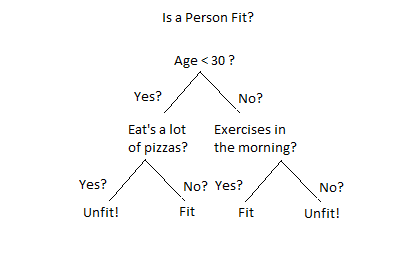
\includegraphics[width=0.5\linewidth]{img/Decision-Trees-modified-1.png}
\end{sectionbox}

\begin{sectionbox}
\subsection{Random Forests}
An ensemble learning method that combines multiple decision trees to create a more robust and accurate model\\
For both classification and regression tasks.

\subsubsection{Assumptions}
\begin{itemize}
    \item None: Like Decision Trees
\end{itemize}

\subsubsection{Architecture}
collections of decision trees
\begin{itemize}
    \item \textbf{Bagging (Bootstrap Aggregating)}: Each tree is trained on a different subset of data, subsets are created by sampling with replacement $\rightarrow$ diversity among trees and minimize overfitting\\
    1. Take a boostrap sample from training data; 2. Build decision tree using this sample
    \item \textbf{Feature Randomness}: standard decision tree: each node, consider all features to find best split $\leftrightarrow$ Random Forest: at each node only a random subset of features, best feature from this subset is used to make the split $\rightarrow$ diversity among trees and more robust
\end{itemize}

\subsubsection{Training Parameters}
\begin{itemize}
    \item Number of Trees: The more trees, the less likely the model will overfit.
    \item Same as decision tree
\end{itemize}

\subsubsection{Use-cases}
\begin{itemize}
    \item Predictive Maintenance
    \item Recommendation Systems
    \item Financial Modeling
\end{itemize}

\begin{tablebox}{p{0.4\textwidth} p{0.55\textwidth}}
\emph{Strengths} & \emph{Weaknesses} \\ \cmrule
High accuracy & Computationally expensive \\
Low overfitting risk & Less interpretable compared to a single decision tree \\
Handles unbalanced datasets well & Not ideal for real-time predictions \\
\end{tablebox}

\subsubsection{Data Preprocessing}
\begin{itemize}
    \item Feature Scaling: Generally not required.
    \item Missing Values: Can handle missing values, but better to impute.
    \item Categorical Variables: Label encoding usually sufficient.
\end{itemize}

\subsubsection{Interpretability}
Moderate; while individual trees are interpretable, the ensemble model complicates interpretation. However, feature importance can still be extracted.
\end{sectionbox}

\begin{sectionbox}
\subsection{Support Vector Machine (SVM)}

Effective for both linear and non-linear classification, regression, and outlier detection.

\subsubsection{Assumptions}
\begin{itemize}
    \item No Noise: Assumes that the data is clean and that there are clear margins of separation.
    \item Two Classes: For basic SVM, the algorithm is inherently binary.
\end{itemize}

\subsubsection{Equation}
The objective is to maximize the margin, defined by \( \frac{2}{\|w\|} \), where \(w\) is the weight vector, subject to constraints \( y_i(w \cdot x_i + b) \geq 1 \).

\subsubsection{Training Parameters}
Kernel: Specifies the type of hyperplane used to separate the data.
\begin{itemize}
    \item Linear Kernel: \(K(x, y) = x \cdot y\)
    \item Polynomial Kernel: \(K(x, y) = (1 + x \cdot y)^d\)
    \item RBF Kernel: \(K(x, y) = e^{-\gamma ||x-y||^2}\)
\end{itemize}
Regularization (C parameter): Balances classification and margin maximization. 

\subsubsection{Use-cases}
\begin{itemize}
    \item Text classification
    \item Image recognition
    \item Bioinformatics (e.g., cancer classification)
\end{itemize}

\begin{tablebox}{p{0.4\textwidth} p{0.55\textwidth}}
\emph{Strengths} & \emph{Weaknesses} \\ \cmrule
High accuracy & Computationally expensive \\
Good for high-dimensional spaces & Sensitive to choice of kernel and regularization \\
Handles non-linear data well & Difficult to interpret \\
\end{tablebox}

\subsubsection{Data Preprocessing}
\begin{itemize}
    \item Feature scaling: Essential due to distance-based optimization.
    \item Missing values: Must be handled prior.
    \item Categorical variables: Ordinal Encoding or One-Hot Encoding.
\end{itemize}

\subsubsection{Interpretability}
Low; the model parameters are hard to interpret in the context of the data, especially for non-linear kernels.

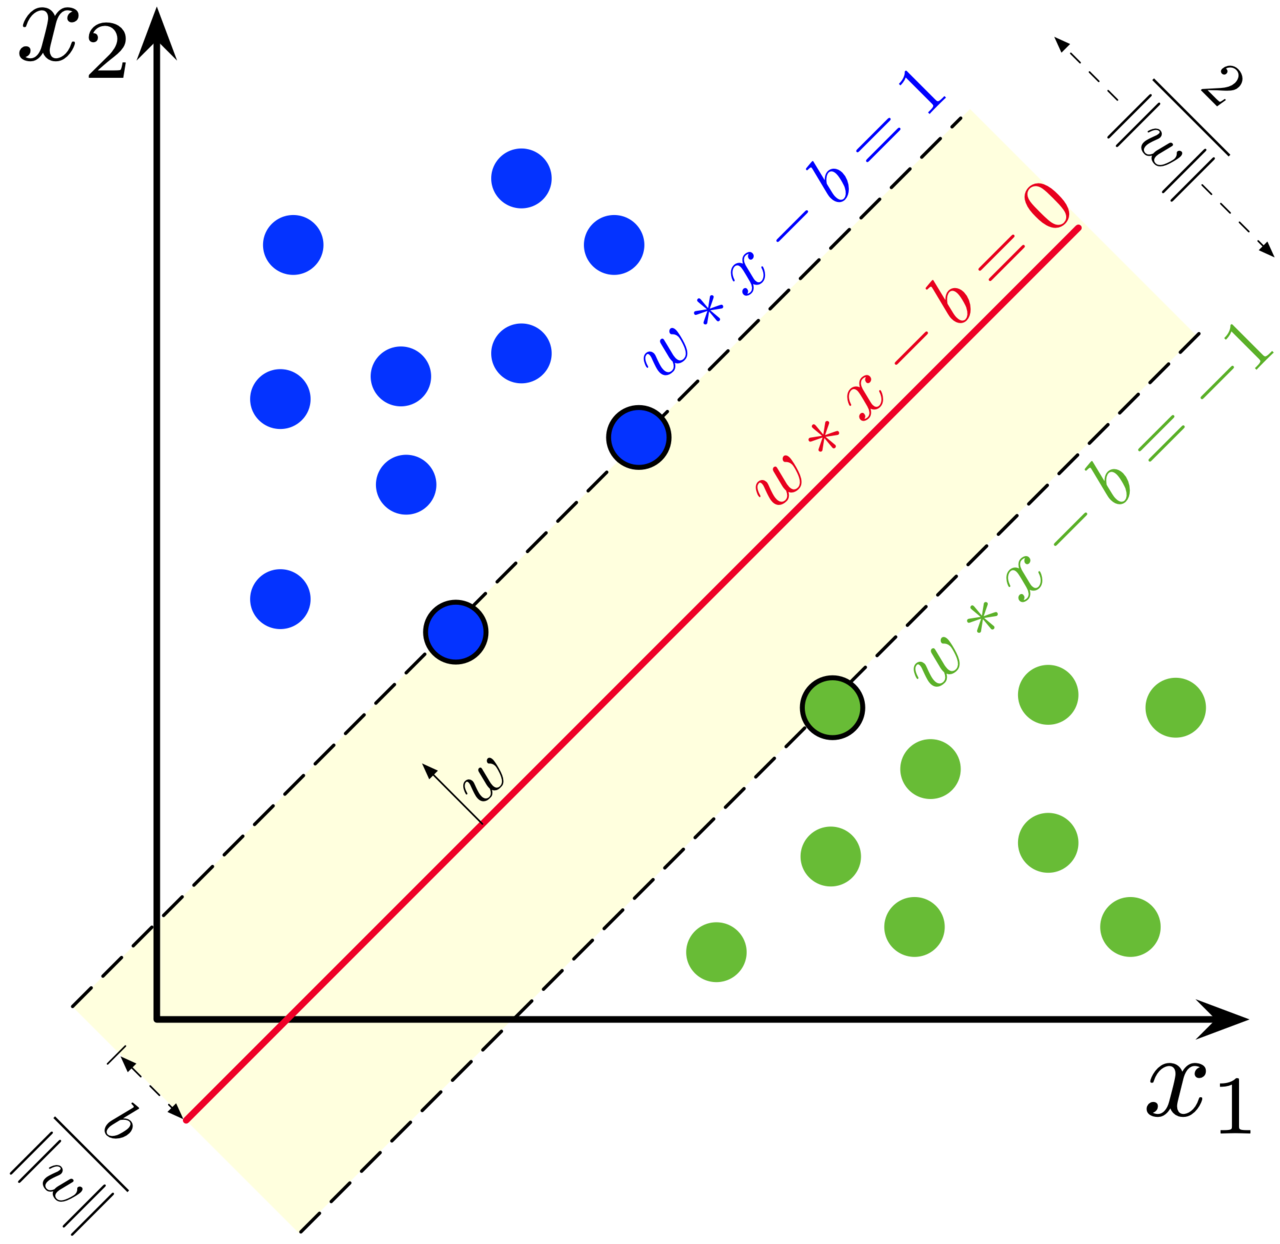
\includegraphics[width=0.3\linewidth]{img/1280px-SVM_margin.png}
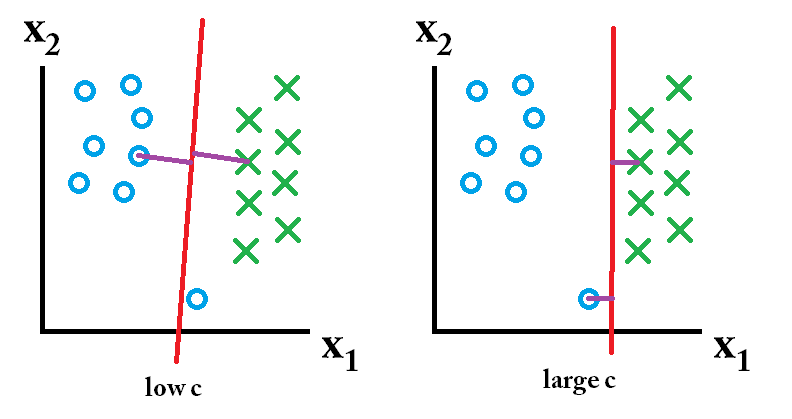
\includegraphics[width=0.5\linewidth]{img/GbW5S.png}
\end{sectionbox}

\begin{sectionbox}
\subsection{k-Nearest Neighbors (k-NN)}

A non-parametric method used for classification and regression tasks based on similarity measures.

\subsubsection{Assumptions}
\begin{itemize}
    \item No underlying model: Assumes no prior knowledge about the underlying data distribution.
    \item Similarity Measure: Assumes similar instances are near each other in the feature space.
\end{itemize}

\subsubsection{Architecture}
Classification is performed by a majority vote among the k-nearest points. Distance measures can include Euclidean, Manhattan, etc.

\subsubsection{Training Parameters}
\begin{itemize}
    \item \( k \): Number of neighbors to consider.
    \item Distance Metric: How to measure the distance between points (e.g., Euclidean, Manhattan).
    \item Weighting: Assign weights to contributions of the neighbors.
\end{itemize}

\subsubsection{Use-cases}
\begin{itemize}
    \item Text categorization
    \item Fraud detection
    \item Recommender systems
\end{itemize}

\begin{tablebox}{p{0.4\textwidth} p{0.55\textwidth}}
\emph{Strengths} & \emph{Weaknesses} \\ \cmrule
Simple to implement & Computationally expensive \\
Adapts easily to multi-class problems & Sensitive to irrelevant features \\
Effective if the feature dimension is low & Requires meaningful distance function \\
\end{tablebox}

\subsubsection{Data Preprocessing}
\begin{itemize}
    \item Feature scaling: Crucial because k-NN uses distance measures.
    \item Missing values: Must be handled; otherwise, they'll impact distance calculations.
    \item Categorical variables: Ordinal Encoding or One-Hot Encoding.
\end{itemize}

\subsubsection{Interpretability}
Moderate; results can be interpreted by examining the closest neighbors, though this becomes harder as dimensionality increases.
\end{sectionbox}

\begin{sectionbox}
\subsection{K-Means Clustering}
An unsupervised learning technique for partitioning data into clusters based on similarity.

\subsubsection{Assumptions}
\begin{itemize}
    \item Distance Metric: Assumes Euclidean distance as a similarity measure.
    \item Spherical Clusters: Assumes clusters to be spherical and equally sized.
\end{itemize}

\subsubsection{Architecture}
Objective is to minimize the sum of squared distances from each point to its cluster centroid.

\[
J = \sum_{i=1}^{k} \sum_{x \in C_i} \|x - \mu_i\|^2
\]

where \(J\) is the objective function, \(C_i\) is the \(i^{th}\) cluster, and \(\mu_i\) is the centroid of \(C_i\).

\paragraph{K-Means}
\begin{enumerate}
    \item Initialize \( k \) cluster centroids randomly or based on some criterion.
    \item Assign each data point to the nearest centroid, and it becomes a member of that cluster.
    \item Recalculate the centroid of each cluster as the mean vector of all points in the cluster.
    \item Repeat steps 2-3 until convergence or a set number of iterations.
\end{enumerate}

\paragraph{K-Means++}
\begin{enumerate}
    \item Choose one centroid uniformly at random from the data points.
    \item For each data point, compute its distance to the nearest, already chosen centroid.
    \item Select the next centroid from the remaining data points with probability proportional to the square of the distance calculated in the previous step.
    \item Repeat steps 2-3 until \( k \) centroids are chosen.
    \item Proceed with steps 2-4 of the standard K-Means algorithm.
\end{enumerate}
\end{sectionbox}

\begin{sectionbox}
\subsubsection{K-Means vs K-Means++}
\begin{itemize}
    \item \textbf{Initialization}: K-Means++ provides a smarter initialization than the random initialization in K-Means.
    \item \textbf{Convergence}: K-Means++ often requires fewer iterations to converge, resulting in performance improvements.
    \item \textbf{Quality}: K-Means++ generally produces clusters with lower intra-cluster variance compared to K-Means.
\end{itemize}

\subsubsection{Training Parameters}
\begin{itemize}
    \item \( k \): Number of clusters.
    \item Initialization: Method for initializing centroids (e.g., random, k-means++).
    \item Max Iterations: Maximum number of iterations for the algorithm to run.
    \item Tolerance: Convergence criteria.
\end{itemize}

\subsubsection{Use-cases}
\begin{itemize}
    \item Market segmentation
    \item Document clustering
    \item Anomaly detection
\end{itemize}

\begin{tablebox}{p{0.4\textwidth} p{0.55\textwidth}}
\emph{Strengths} & \emph{Weaknesses} \\ \cmrule
Simple and fast & Must specify \( k \) in advance \\
Works well for spherical clusters & Sensitive to initial conditions \\
Easily interpretable & Struggles with different cluster sizes \\
\end{tablebox}

\subsubsection{Data Preprocessing}
\begin{itemize}
    \item Feature scaling: Important due to the use of distance metrics.
    \item Missing values: Need to be handled.
\end{itemize}

\subsubsection{Interpretability}
High; centroids and clusters can be easily examined, but interpretation can be subjective.

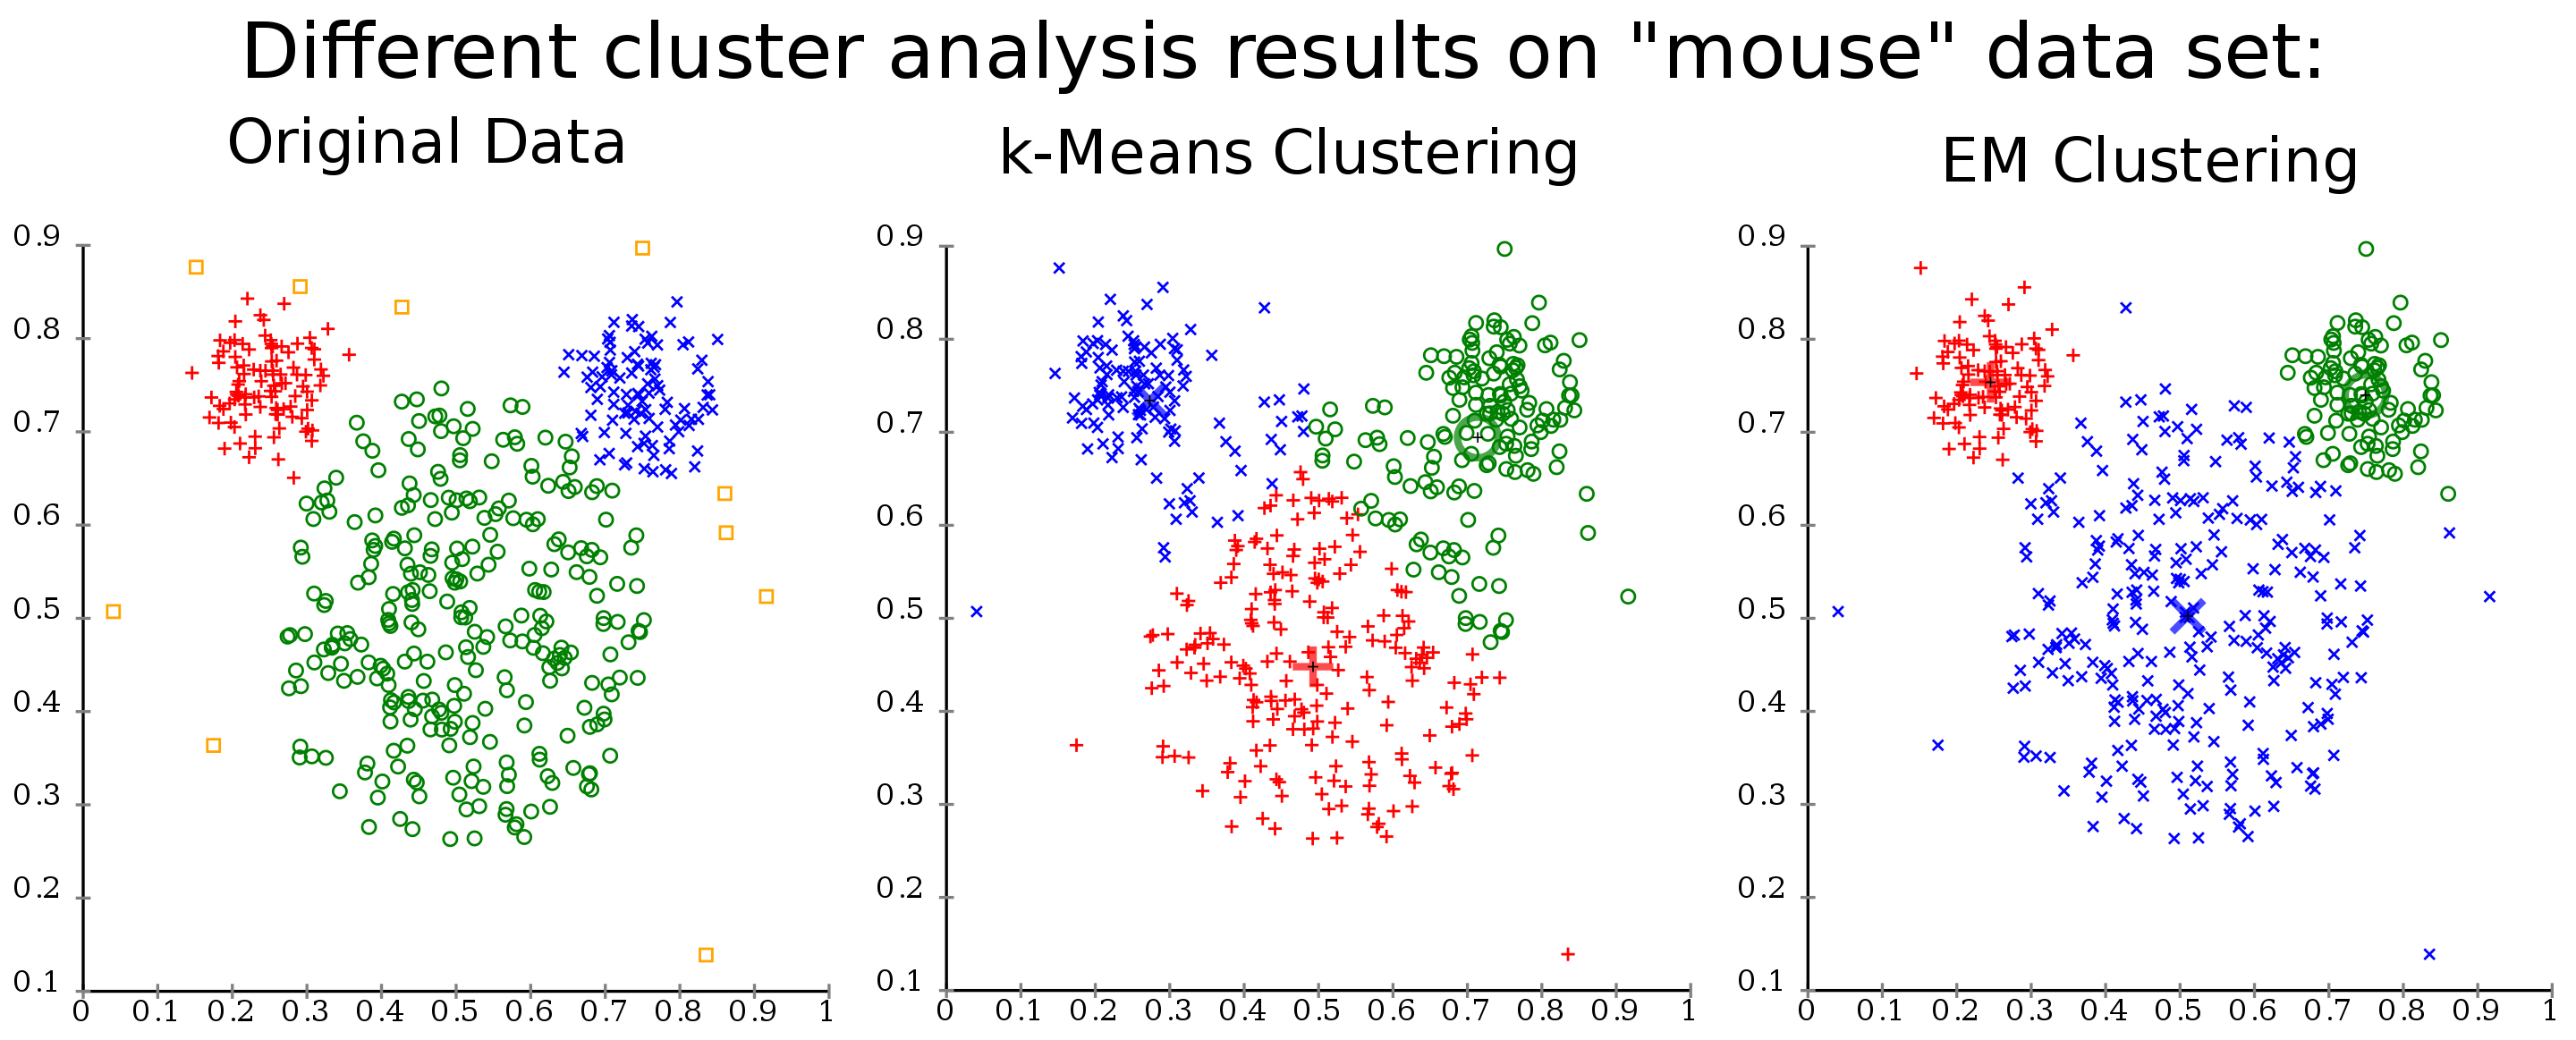
\includegraphics[width=0.9\linewidth]{2880px-ClusterAnalysis_Mouse.svg.png}
\end{sectionbox}

\begin{sectionbox}
\subsection{Hierarchical Clustering}
A clustering algorithm that builds a hierarchy of clusters by either successively merging smaller clusters into larger ones (Agglomerative), or recursively dividing larger clusters into smaller ones (Divisive).

\subsubsection{Assumptions}
\begin{itemize}
    \item No assumptions about the shape or size of the clusters.
    \item Proximity Measures: Various distance metrics can be used (e.g., Euclidean, Manhattan).
\end{itemize}

\subsubsection{Linkage Criteria}
Defines the rule for calculating distance between clusters.
\begin{itemize}
    \item Single Linkage: Minimum distance between clusters.
    \item Complete Linkage: Maximum distance between clusters.
    \item Average Linkage: Average distance between clusters.
    \item Ward's Method: Minimizes the total within-cluster variance.
\end{itemize}

\subsubsection{Algorithm Steps}
\begin{enumerate}
    \item Start with each data point as a single cluster.
    \item Merge the closest pair of clusters based on linkage criteria.
    \item Update the distance matrix.
    \item Repeat steps 2-3 until only one cluster remains.
\end{enumerate}

\subsubsection{Use-cases}
\begin{itemize}
    \item Phylogenetic analysis
    \item Market segmentation
    \item Document clustering
\end{itemize}

\begin{tablebox}{p{0.4\textwidth} p{0.55\textwidth}}
\emph{Strengths} & \emph{Weaknesses} \\ \cmrule
No need to specify number of clusters & Computationally expensive \\
Suitable for non-spherical clusters & Sensitive to choice of linkage criteria \\
Produces a dendrogram, useful for interpretation & No objective way to decide number of clusters \\
\end{tablebox}

\subsubsection{Data Preprocessing}
\begin{itemize}
    \item Feature scaling: Often necessary due to distance metrics.
    \item Missing values: Should be treated carefully.
\end{itemize}

\subsubsection{Interpretability}
High; the dendrogram provides a visual representation and can help understand the nested cluster structure, but choosing the right number of clusters can be subjective.

\end{sectionbox}

\begin{sectionbox}
\subsection{Naive Bayes}

Probabilistic classifiers based on Bayes' theorem, with strong independence assumptions between features.

\subsubsection{Assumptions}
\begin{itemize}
    \item Conditional Independence: Assumes that features are conditionally independent given the class label.
    \item Prior Probability: Requires an estimate of the prior probability of each class.
\end{itemize}

\subsubsection{Equation}
The posterior probability for a class \( C \) given features \( x_1, x_2, \ldots, x_n \) is:
\[
P(C|x_1, x_2, \ldots, x_n) \propto P(C) \prod_{i=1}^{n} P(x_i|C), 
\]
where $P(C)$ is the prior of class C and $P(x_i|C)$ the likelihood

\subsubsection{Training Parameters}
\begin{itemize}
    \item Smoothing: Additive smoothing (Laplace or Lidstone).
    \item Feature Type: Multinomial, Gaussian, or Bernoulli.
\end{itemize}

\subsubsection{Use-cases}
\begin{itemize}
    \item Spam filtering
    \item Sentiment analysis
    \item Document classification
\end{itemize}

\begin{tablebox}{p{0.4\textwidth} p{0.55\textwidth}}
\emph{Strengths} & \emph{Weaknesses} \\ \cmrule
Simple and fast & Assumes feature independence \\
Works well with high dimensions & Sensitive to irrelevant features \\
Effective with small data & Limited to categorical data \\
\end{tablebox}

\subsubsection{Data Preprocessing}
\begin{itemize}
    \item Feature selection: Useful to remove irrelevant features.
    \item Data transformation: Often required for Gaussian Naive Bayes.
\end{itemize}

\subsubsection{Interpretability}
High; easily understandable probabilities and strong assumptions make the model interpretable.
\end{sectionbox}

\begin{sectionbox}
\subsection{Neural Networks}

A class of models inspired by biological neural networks, mainly used for complex pattern recognition and nonlinear function approximation.

\subsubsection{Assumptions}
\begin{itemize}
    \item Universality: Capable of approximating any function given enough neurons.
    \item Data-Driven: Does not impose explicit assumptions on the underlying data distribution.
\end{itemize}

\subsubsection{Equation}
A typical layer in a neural network is defined as:

\[
h = \sigma(Wx + b)
\]

where \( h \) is the output, \( \sigma \) is the activation function, \( W \) is the weight matrix, \( x \) is the input, and \( b \) is the bias.

\subsubsection{Training Parameters}
\begin{itemize}
    \item Learning Rate: Step size in optimization algorithm.
    \item Activation Function: ReLU, Sigmoid, Tanh, etc.
    \item Epochs: Number of times the entire dataset is passed through the network.
    \item Batch Size: Number of samples used in each update.
\end{itemize}

\subsubsection{Use-cases}
\begin{itemize}
    \item Image classification
    \item Natural language processing
    \item Game playing
\end{itemize}

\begin{tablebox}{p{0.4\textwidth} p{0.55\textwidth}}
\emph{Strengths} & \emph{Weaknesses} \\ \cmrule
Highly flexible & Requires large data sets \\
Good for complex tasks & Computationally intensive \\
Self-learning features & Difficult to interpret \\
\end{tablebox}

\subsubsection{Gradient Descent}

An optimization algorithm for minimizing the cost function \( J(\theta) \) iteratively.

\paragraph{Steps}
\begin{enumerate}
    \item \textbf{Initialize Weights}: Randomly initialize model weights \( \theta \).
    \item \textbf{Compute Gradient}: Calculate the gradient \( \nabla J(\theta) \) of the cost function with respect to the weights.
    \[
    \nabla J(\theta) = \frac{1}{m} \sum_{i=1}^{m} \nabla J_i(\theta)
    \]
    \item \textbf{Update Weights}: Update the weights in the opposite direction of the gradient.
    \[
    \theta = \theta - \alpha \nabla J(\theta)
    \]
    where \( \alpha \) is the learning rate.
\end{enumerate}

\subsubsection{Stochastic Gradient Descent (SGD)}

A variant of gradient descent that updates weights after each training example.

\paragraph{Steps}
\begin{enumerate}
    \item \textbf{Initialize Weights}: Randomly initialize model weights \( \theta \).
    \item \textbf{Randomize Data}: Shuffle the training dataset.
    \item \textbf{Compute \& Update}: For each training example \( x_i \), compute the gradient \( \nabla J_i(\theta) \) and immediately update \( \theta \).
    \[
    \theta = \theta - \alpha \nabla J_i(\theta)
    \]
\end{enumerate}

\subsubsection{Comparative Analysis}
\begin{tablebox}{p{0.4\textwidth} p{0.55\textwidth}}
\emph{Strengths} & \emph{Weaknesses} \\ \cmrule
Fast updates & Noisy updates \\
Good for large datasets & May not converge to global minimum \\
Efficient in terms of memory & Sensitive to learning rate \\
\end{tablebox}

\subsubsection{Data Preprocessing}
\begin{itemize}
    \item Feature scaling: Generally required.
    \item Missing values: Not well-suited; must be handled externally.
\end{itemize}

\subsubsection{Interpretability}
Low; often considered as "black-box" models due to their complex structure.
\end{sectionbox}

\begin{sectionbox}
\subsection{Time Series Forecasting}
Using historical data points to predict future observations.

\subsubsection{Characteristics}
\paragraph{Stationarity} Statistical properties like mean and variance are constant over time, often a key issue in time series forecasting.

\paragraph{Seasonality} Patterns that repeat at known intervals (e.g., daily, monthly, annually).

\paragraph{Trend} The underlying trend in the data. Can be upward, downward, or stable.

\paragraph{Cycles} Long-term oscillations driven by economic conditions. Unlike seasonality, the duration is unpredictable.

\paragraph{Autocorrelation} The correlation of a series with its own lags.

\subsubsection{Common Methods}
\paragraph{Exponential Smoothing}
A weighted average method that considers the most recent observations to be more relevant. The simplest form is Simple Exponential Smoothing for univariate time series without trend and seasonality.

\paragraph{ARIMA (AutoRegressive Integrated Moving Average)}
A linear equation that utilizes time-lagged values, lagged forecast errors, and a trend component. Used for non-seasonal time series data.

\textbf{Assumptions:}
\begin{itemize}
    \item Stationarity: Assumes the data is stationary or can be made stationary through differencing.
    \item Linearity: Assumes a linear relationship between lagged variables.
\end{itemize}

\textbf{Equation}
The ARIMA model can be represented as ARIMA\((p, d, q)\), where \(p\) is the AR term, \(d\) is the number of differencing required to make the series stationary, and \(q\) is the MA term.

\[
(1 - \Phi_{1}B - \ldots - \Phi_{p}B^{p}) (1 - B)^{d} Y_{t} = (1 + \theta_{1}B + \ldots + \theta_{q}B^{q}) \epsilon_{t}
\]
\begin{tablebox}{p{0.4\textwidth} p{0.55\textwidth}}
\emph{Strengths} & \emph{Weaknesses} \\ \cmrule
Effective for univariate time-series & Sensitive to parameter choices \\
Handles seasonality with SARIMA & Requires stationary data \\
Good interpretability & Complexity increases with parameters \\
\end{tablebox}

\paragraph{SARIMA (Seasonal ARIMA)}
An extension of ARIMA that explicitly models seasonality. Useful for time series with seasonal components.

\paragraph{Prophet}
An open-source forecasting tool designed for business forecast tasks, providing intuitive parameters to handle trends, seasonality, and holidays.

\subsubsection{Use-cases}
\begin{itemize}
    \item Stock price forecasting
    \item Sales prediction
    \item Weather forecasting
\end{itemize}
\end{sectionbox}

\section{Statistics}
\begin{sectionbox}
\subsection{Descriptive Statistics}
Basic metrics to understand data distributions:
\begin{itemize}
    \item Mean: \(\bar{x} = \frac{1}{N} \sum_{i=1}^{N} x_i\)
    \item Median: Middle value in a sorted list
    \item Mode: Most frequently occurring value
    \item Variance: \(\sigma^2 = \frac{1}{N} \sum_{i=1}^{N} (x_i - \bar{x})^2\)
    \item Standard Deviation: \(\sigma = \sqrt{\sigma^2}\)
\end{itemize}

\subsection{Inferential Statistics}
Tools for making predictions and inferences from sampled data.
\begin{itemize}
    \item Confidence Interval: \( \text{CI} = \bar{x} \pm Z \left( \frac{\sigma}{\sqrt{N}} \right)\)
    \item Hypothesis Testing: Using p-values and significance level (\(\alpha\)) to make decisions.
\end{itemize}

\subsection{Probability Distributions}
Different types of data distributions:
\begin{itemize}
    \item Normal Distribution: \( f(x|\mu, \sigma^2) = \frac{1}{\sqrt{2\pi\sigma^2}} e^{-(x-\mu)^2/(2\sigma^2)} \)
    \item Binomial Distribution: \( f(k, n, p) = C(n, k) p^k (1-p)^{(n-k)} \)
    \item Poisson Distribution: \( P(x; \lambda) = \frac{\lambda^x e^{-\lambda}}{x!} \)
\end{itemize}

\subsubsection{Probability Formulas}
\begin{itemize}
    \item Probability: \( P(A) = \frac{\text{Number of favorable outcomes}}{\text{Total number of outcomes}} \)
    \item Conditional Probability: \( P(A|B) = \frac{P(A \cap B)}{P(B)} \)
    \item Bayes' Theorem: \( P(A|B) = \frac{P(B|A)P(A)}{P(B)} \)
\end{itemize}
\vspace{\baselineskip}
\begin{itemize}
    \item Expected Value: \( E(X) = \sum_{i=1}^{n} p(x_i) x_i \)
    \item Variance: \( \text{Var}(X) = E(X^2) - [E(X)]^2 \)
    \item Standard Deviation: \( \sigma = \sqrt{\text{Var}(X)} \)
\end{itemize}
\vspace{\baselineskip}
\begin{itemize}
    \item Covariance: \( \text{Cov}(X, Y) = \frac{1}{N} \sum_{i=1}^{N} (x_i - \bar{x})(y_i - \bar{y}) \)
    \item Pearson Correlation Coefficient: \( r = \frac{\text{Cov}(X, Y)}{\sigma_x \sigma_y} \)
\end{itemize}
\end{sectionbox}


\section{Other}
\begin{sectionbox}
\subsection{Multiclass Prediction}
Output variable can take on more than two classes, aims to assign an observation to one of several classes. 

\begin{itemize}
    \item \textbf{One-vs-All (OvA)}: 
    \begin{itemize}
        \item \textit{Method}: For \(N\) classes, \(N\) separate binary classifiers are trained. Each one discriminates between one of the classes and the rest.
        \item \textit{Advantages}: Simplicity and ease of implementation.
    \end{itemize}
    
    \item \textbf{One-vs-One (OvO)}:
    \begin{itemize}
        \item \textit{Method}: For \(N\) classes, \( \binom{N}{2} \) classifiers are trained, one for each pair of classes.
        \item \textit{Advantages}: Each classifier needs only to be trained on the subset of the data containing its two target classes, potentially providing more accurate results.
    \end{itemize}

    \item \textbf{Softmax Regression}:
    \begin{itemize}
        \item \textit{Method}: Generalizes logistic regression to multiple classes without requiring multiple binary classifiers.
        \item \textit{Advantages}: Provides probabilities for each class, useful for interpretability.
    \end{itemize}
    
    \item \textbf{Tree-based Methods}:
    \begin{itemize}
        \item \textit{Method}: Decision trees or ensemble methods like Random Forest can naturally handle multiclass classification.
        \item \textit{Advantages}: Interpretability and handling of missing values.
    \end{itemize}
\end{itemize}

\end{sectionbox}

\begin{sectionbox}
\subsection{Dimensionality Reduction}
Techniques to reduce the number of features while preserving the underlying data structure. Useful for visualization, reducing noise, and improving model performance.

\subsubsection{Principal Component Analysis (PCA)}
\begin{itemize}
    \item Objective: To find orthogonal axes (principal components) that maximize the variance.
    \item Algorithm: Eigen-decomposition of the covariance matrix.
    \item Use-cases: Image compression, visualization, feature extraction.
\end{itemize}

\paragraph{Steps}
\begin{enumerate}
    \item \textbf{Standardize Data}: Scale the data to have zero mean and unit variance.
    \[
    X_{\text{std}} = \frac{X - \mu}{\sigma}
    \]
    
    \item \textbf{Compute Covariance Matrix}: Calculate the covariance matrix of the standardized data.
    \[
    \Sigma = \frac{1}{n} X_{\text{std}}^T X_{\text{std}}
    \]
    
    \item \textbf{Eigenvalue Decomposition}: Calculate the eigenvalues and eigenvectors of the covariance matrix.
    \[
    \Sigma v = \lambda v
    \]
    
    \item \textbf{Sort Eigenvalues}: Sort the eigenvalues in descending order and select the top \(k\) corresponding eigenvectors.
    
    \item \textbf{Projection}: Project the original data onto the lower-dimensional subspace.
    \[
    X_{\text{pca}} = X_{\text{std}} \times W
    \]
    where \(W\) is the matrix formed by the top \(k\) eigenvectors.
\end{enumerate}

\subsubsection{Linear Discriminant Analysis (LDA)}
\begin{itemize}
    \item Objective: To find a linear combination of features that maximizes the separation between different classes.
    \item Algorithm: Maximizes the ratio of between-class variance to within-class variance.
    \item Use-cases: Classification, feature extraction.
\end{itemize}
\paragraph{Steps}
\begin{enumerate}
    \item \textbf{Compute Class Means}: Calculate the mean vectors for each class.
    \[
    \mu_i = \frac{1}{n_i} \sum_{x \in C_i} x
    \]
    
    \item \textbf{Within-class Scatter Matrix \(S_W\)}:
    \[
    S_W = \sum_{i=1}^{c} \sum_{x \in C_i} (x - \mu_i) (x - \mu_i)^T
    \]
    
    \item \textbf{Between-class Scatter Matrix \(S_B\)}:
    \[
    S_B = \sum_{i=1}^{c} n_i (\mu_i - \mu) (\mu_i - \mu)^T
    \]
    where \(\mu\) is the overall mean.
    
    \item \textbf{Eigenvalue Decomposition}: Solve the generalized eigenvalue problem for \(S_W^{-1} S_B\).
    \[
    S_W^{-1} S_B v = \lambda v
    \]
    
    \item \textbf{Sort Eigenvalues}: Sort the eigenvalues in descending order and select the top \(k\) corresponding eigenvectors.
    
    \item \textbf{Projection}: Project the original data onto the lower-dimensional subspace.
    \[
    X_{\text{lda}} = X \times W
    \]
    where \(W\) is the matrix formed by the top \(k\) eigenvectors.
\end{enumerate}
\end{sectionbox}

\begin{sectionbox}
\subsubsection{Factor Analysis}
\begin{itemize}
    \item Objective: To model observed variables as linear combinations of latent variables and error terms.
    \begin{equation*}
    \begin{array}{c}
    \underset{\mathrm{p \times n}}{
        \overset{\text{data}}{
            \left[
            \begin{array}{l}
            \textcolor{red}{\text{math scores}} \\
            \textcolor{blue}{\text{reading scores}} \\
            \textcolor{green}{\text{science scores}}
            \end{array}
            \right]
        }
    }
    =
    \underset{\mathrm{p \times k}}{
        \overset{\text{factor loadings}}{
            \left[
            \begin{array}{rr}
            \textcolor{purple}{.13} & \textcolor{cyan}{.95} \\
            \textcolor{purple}{.78} & \textcolor{cyan}{-.28} \\
            \textcolor{purple}{-.87} & \textcolor{cyan}{.05}
            \end{array}
            \right]
        }
    }
    \underset{\mathrm{k \times n}}{
        \overset{\text{common factors}}{
            \left[
            \begin{array}{cccc}
            \textcolor{purple}{-1.25} & \textcolor{purple}{1.88} & \ldots & \textcolor{purple}{-0.55} \\
            \textcolor{cyan}{0.71} & \textcolor{cyan}{-0.17} & \ldots & \textcolor{cyan}{-1.20}
            \end{array}
            \right]
        }
    } \\
    \end{array}
    \end{equation*}

    \item Algorithm: Factor loadings are estimated through methods like maximum likelihood.
    \item Use-cases: Psychology tests, market research, gene expression data.
\end{itemize}

\begin{tablebox}{p{0.4\textwidth} p{0.55\textwidth}}
\emph{Strengths} & \emph{Weaknesses} \\ \cmrule
Reduces overfitting & Loss of interpretability \\
Speeds up training & Assumes linear relationships \\
Improves model generalization & May lose important features \\
\end{tablebox}

\subsubsection{Data Preprocessing}
\begin{itemize}
    \item Feature scaling: Mandatory for most algorithms due to distance computation.
    \item Handling missing values: Impute or remove rows/columns.
\end{itemize}

\subsubsection{Interpretability}
Medium; interpreting reduced dimensions may be non-intuitive but techniques like loading plots can help.

\end{sectionbox}

\begin{sectionbox}
\subsection{Hypothesis Testing in A/B Testing}
\subsubsection{Steps}
\begin{enumerate}
    \item \textbf{Null Hypothesis (\(H_0\))}: Assume that there is no difference between the performance of model A and model B.
    \item \textbf{Alternative Hypothesis (\(H_a\))}: Assume that there is a significant difference between the performance of model A and model B.
    \item \textbf{Choose Significance Level (\(\alpha\))}: Commonly set at 0.05, implying a 95\% confidence level.
    \item \textbf{Collect Data}: Record the performance metric for both groups over a set period.
    \item \textbf{Calculate Test Statistic}: This could be a t-statistic, z-score, etc., depending on the data distribution.
    \item \textbf{Compute P-value}: The probability of observing the data if the null hypothesis were true.
    \item \textbf{Draw Conclusions}:
    \begin{itemize}
        \item If \( p \leq \alpha \), reject the null hypothesis. This suggests that the difference in performance is statistically significant.
        \item If \( p > \alpha \), fail to reject the null hypothesis. This suggests that the difference in performance is not statistically significant.
    \end{itemize}
\end{enumerate}

\subsubsection{Important Notes}
\begin{itemize}
    \item A smaller p-value suggests stronger evidence against the null hypothesis.
    \item Rejecting the null hypothesis does not prove the alternative hypothesis; it only suggests that the alternative hypothesis is more likely.
    \item Hypothesis testing only indicates if a difference exists, not the magnitude of the difference.
\end{itemize}

\end{sectionbox}

% ======================================================================
% End
% ======================================================================
\end{document}
